\section{فرمول‌های ریاضی}
\begin{frame}[fragile]{نوشتن فرمول‌های پیچیده ریاضی}
\begin{latin}
\begin{lstlisting}[keywords={begin, end}, keywordstyle=\color{Mulberry}\textbf, numbers=none]
\begin{equation*}
    \Rightarrow
        \begin{split}
        \vec{r}\,(r, \theta) & = (r\cos\theta, r\sin\theta, r) \\
        \vec{r}_r & = (\cos\theta, \sin\theta, r) \\
        \vec{r}_\theta & = (-r\sin\theta, r\cos\theta, 0) \\
    \end{split}
\end{equation*}
\end{lstlisting}
\end{latin}
\end{frame}


\begin{frame}[fragile]{نوشتن فرمول‌های پیچیده ریاضی}
\begin{latin}
\begin{lstlisting}[keywords={begin, end}, keywordstyle=\color{Mulberry}\textbf, numbers=none]
\begin{equation*}
    \Rightarrow
    \vec{r}_r \times \vec{r}_\theta = 
    \begin{vmatrix}
        i & j & k \\
        \cos\theta & \sin\theta & r \\
        -r\sin\theta & r\cos\theta & 0 
    \end{vmatrix} = (-r\cos\theta, -r\sin\theta, r)
\end{equation*}
\end{lstlisting}
\end{latin}
\end{frame}

\begin{frame}[fragile]{نوشتن فرمول‌های پیچیده ریاضی}
\begin{latin}
\begin{lstlisting}[keywords={begin, end}, keywordstyle=\color{Mulberry}\textbf, numbers=none]
\begin{equation*}
    \Rightarrow
    \left|\vec{r}_r \times \vec{r}_\theta\right|
    = \sqrt{
    \underbrace{
        (r^2\cos^2\theta) +
        (r^2\sin^2\theta)
    }_{=r^2}
        + r^2
    }
    = \sqrt{2r^2}
    = r\sqrt{2} 
\end{equation*}
\end{lstlisting}
\end{latin}
\end{frame}

\begin{frame}{خروجی}
\begin{center}
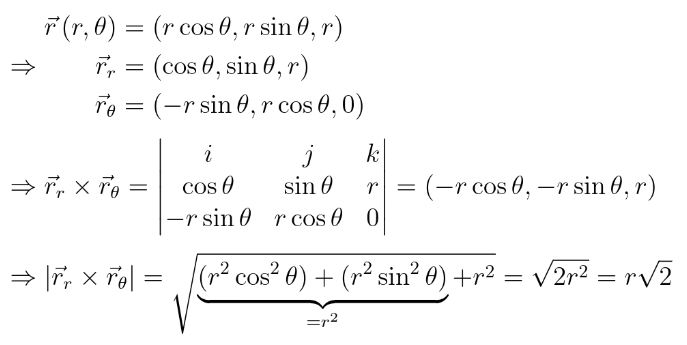
\includegraphics[width=0.8\textwidth]{docs/images/math1}
\end{center}
\end{frame}
